%
% Frontmatter - Introducci�n. Los miembros del tribunal que juzgan los PFC's tienen muchas m�s memorias que leer, por lo que
%	agradecer�n cualquier detalle que permita facilitarles la vida. En este sentido, realizar una peque�a introducci�n,
%	comentar la organizaci�n y estructura de la memoria y resumir brevemente cada cap�tulo puede ser una buena pr�ctica
%	que permita al lector centrarse f�cilmente en la parte que m�s le interesa.
%

\chapter[Introduction]{
	Introduction
}

Computer Vision is a field that includes techniques for acquiring, processing, analyzing, and understanding images. This scientific area is not only limited to images but also to high-dimensional data from the real world. It aims to produce numerical or symbolic information in order to perform decisions \cite{computervision}. A common trend in this field, has been duplicating the abilities of human vision by electronically perceiving and interpreting the image. 

\begin{figure}[h]
	\centering
	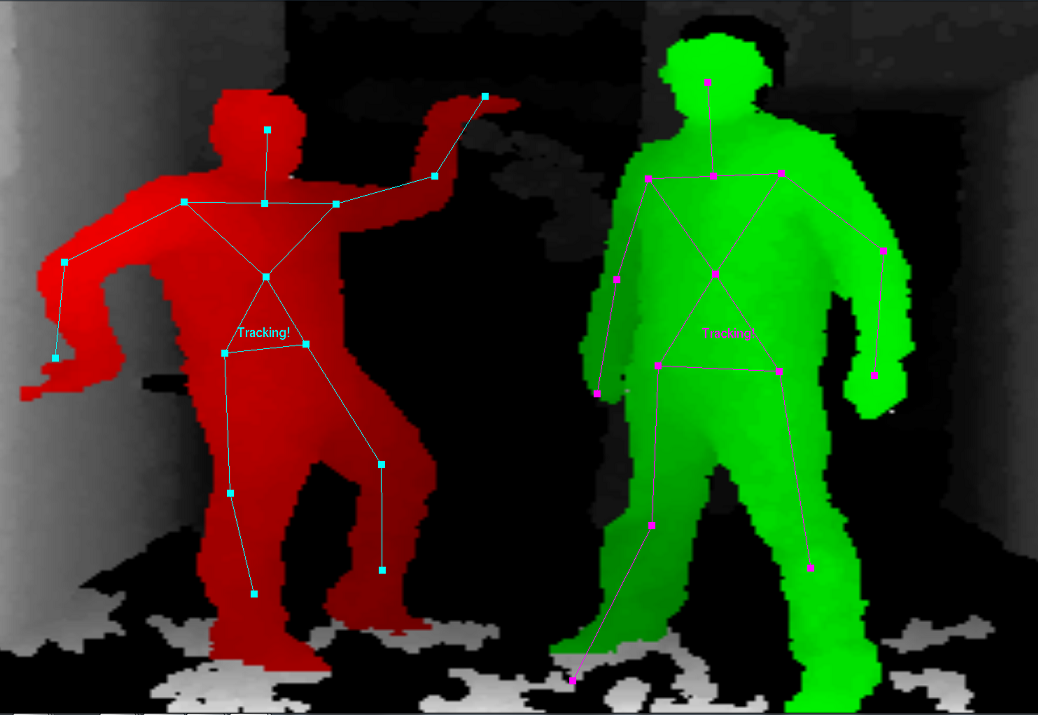
\includegraphics[scale=0.4]{figures/pose_estimation.png}
	\caption[Pose estimation]{
		The specific task of determining the pose of an object in an image is referred to as pose estimation.
	}
	\label{pose_estimation}
\end{figure}

This image understanding can be seen as the extraction of symbolic information from image data using models constructed with the aid of geometry, physics, statistics, and learning theory \cite{computervisionmodern}. As a scientific discipline, Computer Vision considers the theory behind artificial systems that extract information from images. The image data can have many forms, such as video frames, views from multiple cameras, or multi-dimensional data from a medical scanner. As a technological discipline, Computer Vision seeks to apply its theories and models to the construction of artificial vision systems.

Sub-domains of computer vision include scene reconstruction, event detection, video tracking, object recognition, object pose estimation, learning, indexing, motion estimation, and image restoration (see \figurename~\ref{pose_estimation}). Our case study pertains to the field of stereo vision. In this subject, the main objective is the extraction of 3D information from digital images, such as obtained by a CCD camera. By comparing information about a scene from two vantage points, 3D data can be extracted by examination of the relative positions of objects in the two panels (see \figurename~\ref{stereoscopic_vision}).

\begin{figure}[h]
  \centering
  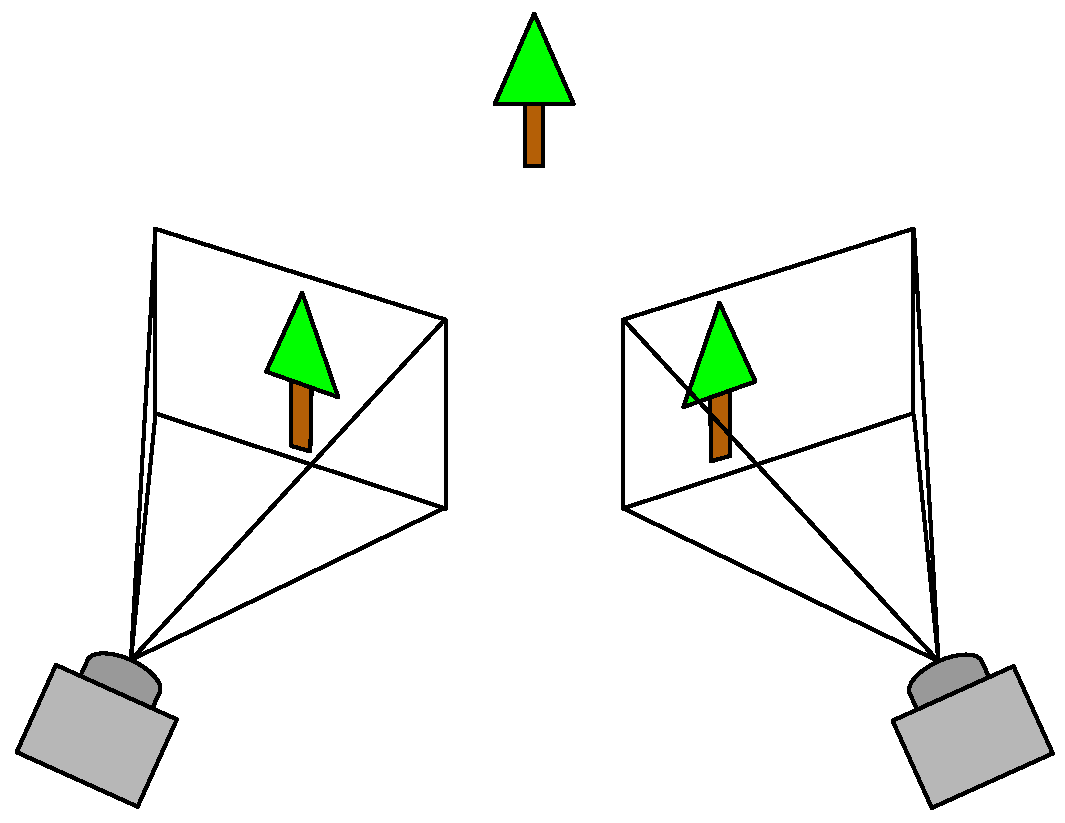
\includegraphics[width=0.475\textwidth]{figures/stereo.pdf} \quad
  \caption[Stereoscopic vision]{
  		Basic diagram of a stereo vision setup.
  	}
  \label{stereoscopic_vision}
\end{figure} 

\section[Motivation and context]{
	Project motivation and context
}

One of the key steps in stereo vision techniques, is obtaining the stereo correspondence between two images or Stereo Matching. The correspondence problem refers to the process of ascertaining which parts of one image correspond to which parts of another image. This is not a trivial affair, since differences appear due to movement of the camera, the elapse of time, and/or movement of objects in the photos.

Current approaches to obtain this information, involve the usage of a single CPU. Our aim with this project is taking advantage of modern hardware to its fullest capacities. This is specially important nowadays, since camera systems keep on improving leading to images with very high resolutions. This complex task involves exploiting the massive parallel power of current multi-core CPUs, GPUs, etc. In addition, our desire is not only the implementation of a Stereo Matching algorithm; but the creation of a \CC framework that will allow the user to implement parallel Computer Vision algorithms with ease.

The set of software tools developed in this project has been called \textbf{GCVL} (GPU Computer Vision Library). This library provides several means to implement GPU algorithms in an simpler manner using OpenCL or CUDA. In addition, a sample implementation of a Stereo Matching algorithm called Block Matching will also be provided to showcase the features offered in the framework. This algorithm will have a serial, OpenMP, OpenCL and CUDA implementation that employs the designed software tools.     

\section[Objectives]{
	Project objectives
}

The main objectives in this project are:

\begin{itemize}
\item Studying different Stereo Matching techniques.
\item Design, implementation and documentation of tools to ease GPGPU programming.
\item Design, implementation and documentation of the chosen algorithm. 
\item CPU parallelization of the implemented algorithm.
\item GPU parallelization of the implemented algorithm.
\end{itemize}

In this project, a fast Stereo Matching algorithm is required. In addition, the algorithm needs to keep all the precision possible, but be suitable for real-time processing of interactive image sequences. Not only this, but also the algorithm needs to be highly parallel so GPUs can be efficiently used. This algorithm will be implemented with the developed toolset for GPGPU computing. Moreover, evidence will be collected of the scalability and performance of the chosen algorithm and its parallel implementations.

\section[Structure]{
Document structure
}

The rest of the document is organized following this structure:

\paragraph*{Chapter 2.}
Technological Foundations

This chapter briefs very basic concepts about Computer Vision needed to understand the rest of the document: How stereo correspondence, stereo matching and our chosen solution work. This chapter will also introduce the reader to basic GPGPU concepts.

\paragraph*{Chapter 3.}
GCVL: GPGPU Computer Vision Library

This chapter describes the structure of the library we propose in this work and presents the class diagram of the software package.
 
\paragraph*{Chapter 4.}
Performance \& Experimental Results

This chapter presents the obtained performance and experimental results, so that the reader can compare our parallel implementations with the sequential one.

\paragraph*{Chapter 5.}
Conclusions and future lines of work

Finally, this chapter presents the main conclusions obtained with this
project and outlines possible extensions to GCVL.
